\chapter{Einleitung}
\label{ch:einleitung}

\section{Problemstellung}
\label{sec:motivation}
WAS SOLL IN DER MASTERARBEIT BEHANDELT WERDEN?

Das Konzept der vorausschauenden Wartung (eng. \textit{predictive Maintenance (PDM)}) ist nicht neu. Schon im vergangenen Jahrhundert wurden Methoden entwickelt, um an hand von Messwerten Schlüsse über den Betriebszustand einer Maschine zu ziehen. Beispielsweise konnte so der Verschleißzustand von Lokomotiven anhand von Ölproben bestimmt werden. \todo{Mehr Researche nötig} Dennoch war und ist PDM auch heute noch nur in wenigen Einsatzgebieten gängige Praxis.

Mit dem Aufschwung der Industrie 4.0 und der damit einhergehenden stetig größer weredenden Menge verfügbarer Daten, rückt PDM jedoch aus Nischenanwendungen aktuell weiter in den Fokus von Anlagenbetreidenden. Schließlich bieten sich durch eine große Menge Daten neue Möglichkeiten. Nicht nur können bestehende Anwendungen mit größerer Präzision ausgeführt werden; es ergeben sich auch grundlegend neue Anwendungsmöglichkeiten. \todo{Beispiel}

PDM ist in vielen technischen Bereichen insbesondere deshalb interessant, weil  dadurch nach Hölzel folgende Potentiale erschlossen werden können \todo{Verweis auf Hölzel S.31}. Diese sind in abgrenzung zur präventativen Instandhaltung zu sehen:
\begin{itemize}
	\item Bedarfsgerechte Ersatzteilbereitstellung
	\item Instandhaltungsmaßnahmen können zum optimalen Zeitpunkt durchgeführt werden
	\item Verlängerung der anlagen- und Bauteillebensdauer
	\item Reduzierte Stillstandzeiten
	\item Reduzierte Instandhaltungskosten
	\item Verbesserung der Anlagenzuverlässigkeit
\end{itemize}

Auch für die Instandhaltung von Schienenfahrzeugen erscheinen PDM-Anwendungen interessant. Neben den oben genannten Punkten scheint sich durch die Verringerung von Ausfällen auch Imageschaden abzuwenden. Dieser Entsteht, wenn  der Ausfall einer Anlage sich direkt auf den Kunden auswirkt; in diesem Fall der Fahrgast.

Ein häufig beobachteter Fall sind Türstörungen. In der Regel äußern sich diese darin, dass die Zugtür nicht mehr entsprechend der Sicherheitsanforderungen nutzbar sind. In den meisten Fällen genügt es jedoch die Tür außer Betrieb zusetzen und um so die Sperrung eines Waggons oder gar den Ausfall einer ganzen Fahrt zu verhindern. Dennoch ist der Ausfall einer Zugtür für den Kunden direkt ersichtlich und führt damit zu einem Imageschaden. Aus diesem Grund erscheint der Einsatz vorausschauender Wartung auch hier sinnvoll, obwohl aus technisch wirtschaftlicher Sicht eine Instandhaltung nach präventiven Methoden ausreichend wäre. 

Die Fragestellung die bei der Umsetzung aller PDM-Anwendungen zunächst geklärt werden muss ist, ob das entwickelte Modell zur Vorhersage ausreichend präzise Vorhersagen trifft. Insbesondere entscheidend ist dabie der vergleich mit der gegenwärtigen Instandhaltungsstrategie.

\begin{figure}[ht]
	\centering
	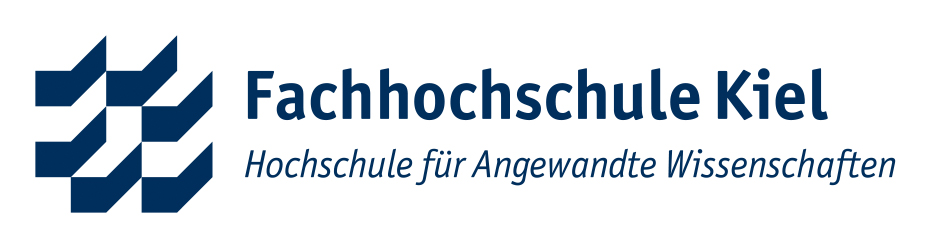
\includegraphics[scale=0.4]{FH_Kiel_Logo_deut_rgb.jpg}
	\caption{Logo}
	\label{fig:fhlogo}
\end{figure}

dskalfj dsaflke dsd dkslf ssfe e dsd dkslf ssfe dsfafeklflsdkf
\section{Ziel der Arbeit}
\label{sec:ziel}
WELCHE ERGEBNISSE UND ERKENNTNISSE SOLLEN AM ENDE FESTSTEHEN?

Kern dieser Arbeit ist es ein maschinelles Lernmodel für einen PDM-Usecase zu entwickeln. Das zugrunde leigende Instandhaltungsproblem ist dabei eine Beschädigte aber noch funktionstüchtige Umlenkrolle. Abschließend soll die Tauglichkeit des Modell für einen fiktiven PDM-Usecase bewertet werden. 



Das Modell soll in der Lage sein Beschädigungen einer Umlenkrolle zu erkennen. Die Umlenkrolle mit dem ein simulierter Schadenfall vorhergesagt werden könnte. Die Arbeit ist dabei vor der Vision angesiedelt maschinelle Lernverfahren für die vorausschauende Instandhaltung einzusetzten. Entsprechend sollen die Ergebnisse der Modelentwicklung vor diesem Hintergrund beleuchtet werden.

\section{Vorgehensweise}
\label{sec:vorgehensweise}
WELCHE SCHRITTE WERDEN DURCHLAUFEN UM DIE ANGESTREBTEN ERGEBNISSE ZU ERHALTEN?
(LÄSST SICH NACH KAPITELN ORDNEN)
- anforderungen an PDm-usecase definieren und Score-Formel ableiten
- Datensatz aufnehmen
- Modelle trainieren
- Model-Scores vergeben 